\batchmode
\documentclass{report}
\RequirePackage{ifthen}


\usepackage{amssymb}
\usepackage[dvips]{graphicx}
\usepackage{verbatim}
\usepackage{html}


\usepackage{amsmath}
\usepackage{latexsym,amssymb}
\usepackage[mathscr]{eucal}
\usepackage{amsthm,amsxtra,amscd,upref}
\usepackage{layout,bm,dcolumn}
\usepackage{graphicx,color}
\usepackage{calc}


\usepackage{framed}

%
\providecommand{\DST}[1]{{\ensuremath{\displaystyle{#1}}}}%
\providecommand{\DSF}[2]{{\ensuremath{\displaystyle{\frac{{\ensuremath{\displaystyle{#1}}}}{{\ensuremath{\displaystyle{#2}}}}}}}} 

%
\providecommand{\vk}[1]{{\ensuremath{\underline{\bm{#1}}}}}%
\providecommand{\mx}[1]{{\ensuremath{\bm{\mathsf{#1}}}}}%
\providecommand{\lrb}[1]{{\ensuremath{\left({#1}\right)}}}%
\providecommand{\lrs}[1]{{\ensuremath{\left[{#1}\right]}}}%
\providecommand{\lrc}[1]{{\ensuremath{\left\{{#1}\right\}}}}%
\providecommand{\lrv}[1]{{\ensuremath{\left|{#1}\right|}}} 

%
\providecommand{\hell}{{\ensuremath{\hat{\jmath}}}}%
\providecommand{\zell}{{\ensuremath{\mathfrak{z}}}}%
\providecommand{\vM}{{\ensuremath{{\ensuremath{\underline{\bm{M}}}}}}}%
\providecommand{\vr}{{\ensuremath{{\ensuremath{\underline{\bm{r}}}}}}}%
\providecommand{\vq}{{\ensuremath{{\ensuremath{\underline{\bm{q}}}}}}}%
\providecommand{\vh}{{\ensuremath{{\ensuremath{\underline{\bm{h}}}}}}}%
\providecommand{\vkx}{{\ensuremath{{\ensuremath{\underline{\bm{x}}}}}}}%
\providecommand{\vkxt}{{\ensuremath{{\ensuremath{\underline{\bm{x}}}}^t}}}%
\providecommand{\vky}{{\ensuremath{{\ensuremath{\underline{\bm{y}}}}}}}%
\providecommand{\vkyt}{{\ensuremath{{\ensuremath{\underline{\bm{y}}}}^t}}} 

%
\providecommand{\vri}[1]{{\ensuremath{{\ensuremath{\underline{\bm{r}}}}_{#1}}}}%
\providecommand{\vrr}{{\ensuremath{{\ensuremath{\underline{\bm{r}}}}}}}%
\providecommand{\vqi}[1]{{\ensuremath{{\ensuremath{\underline{\bm{q}}}}_{#1}}}}%
\providecommand{\vqr}{{\ensuremath{{\ensuremath{\underline{\bm{q}}}}}}}%
\providecommand{\vhi}[1]{{\ensuremath{{\ensuremath{\underline{\bm{h}}}}_{#1}}}}%
\providecommand{\vhr}{{\ensuremath{{\ensuremath{\underline{\bm{h}}}}}}}%
\providecommand{\IMA}{{\ensuremath{\mathrm{i}}}}%
\providecommand{\EE}{{\ensuremath{\mathrm{e}}}}%
\providecommand{\half}{{\ensuremath{\frac{1}{2}}}} 

%
\providecommand{\deltax}{{\ensuremath{\rho\cos(\beta)}}}%
\providecommand{\deltay}{{\ensuremath{\rho\sin(\beta)}}}%
\providecommand{\deltaz}{{\ensuremath{\delta_{z}}}}%
\providecommand{\deltazs}{{\ensuremath{\widehat{{\ensuremath{\delta_{z}}}}}}}%
\providecommand{\DD}[1]{{\ensuremath{\mathrm{d}{#1}\, }}}%
\providecommand{\DDD}[2]{{\ensuremath{\mathrm{d}^{#1}{#2}\, }}} 

%
\providecommand{\haf}{{\ensuremath{\scriptstyle{\frac{1}{2}}}}}%
\providecommand{\unt}{{\ensuremath{\scriptstyle{\frac{1}{3}}}}}%
\providecommand{\dut}{{\ensuremath{\scriptstyle{\frac{2}{3}}}}}%
\providecommand{\xref}[1]{(\ref{#1})}%
\providecommand{\eref}[1]{Eq.~(\ref{#1})}%
\providecommand{\Beref}[1]{{\textcolor[rgb]{0,0,1}{Eq.~(\ref{#1})}}}%
\providecommand{\eeref}[2]{Eqs.~(\ref{#1},\ref{#2})}%
\providecommand{\eeeref}[3]{Eqs.~(\ref{#1},\ref{#2},\ref{#3})}%
\providecommand{\aref}[1]{Appendix~\ref{#1}}%
\providecommand{\sref}[1]{Sec.~\ref{#1}}%
\providecommand{\cref}[1]{Chap.~\ref{#1}}%
\providecommand{\tref}[1]{Tab.~\ref{#1}}%
\providecommand{\fref}[1]{Fig.~\ref{#1}}%
\providecommand{\Rref}[1]{Ref.~\cite{#1}}%
\providecommand{\degC}{{\ensuremath{{}^{\mathrm{o}}}}} 

%
\providecommand{\TT}{{\ensuremath{{2\theta}}}}%
\providecommand{\TTz}{{\ensuremath{{{{\ensuremath{{2\theta}}}}_{0}}}}}%
\providecommand{\TTe}{{\ensuremath{{{{\ensuremath{{2\theta}}}}_{e}}}}}%
\providecommand{\TTB}{{\ensuremath{{{{\ensuremath{{2\theta}}}}_{B}}}}} 





\pagecolor[gray]{.7}

\usepackage[]{inputenc}



\makeatletter

\makeatletter
\count@=\the\catcode`\_ \catcode`\_=8 
\newenvironment{tex2html_wrap}{}{}%
\catcode`\<=12\catcode`\_=\count@
\newcommand{\providedcommand}[1]{\expandafter\providecommand\csname #1\endcsname}%
\newcommand{\renewedcommand}[1]{\expandafter\providecommand\csname #1\endcsname{}%
  \expandafter\renewcommand\csname #1\endcsname}%
\newcommand{\newedenvironment}[1]{\newenvironment{#1}{}{}\renewenvironment{#1}}%
\let\newedcommand\renewedcommand
\let\renewedenvironment\newedenvironment
\makeatother
\let\mathon=$
\let\mathoff=$
\ifx\AtBeginDocument\undefined \newcommand{\AtBeginDocument}[1]{}\fi
\newbox\sizebox
\setlength{\hoffset}{0pt}\setlength{\voffset}{0pt}
\addtolength{\textheight}{\footskip}\setlength{\footskip}{0pt}
\addtolength{\textheight}{\topmargin}\setlength{\topmargin}{0pt}
\addtolength{\textheight}{\headheight}\setlength{\headheight}{0pt}
\addtolength{\textheight}{\headsep}\setlength{\headsep}{0pt}
\setlength{\textwidth}{349pt}
\newwrite\lthtmlwrite
\makeatletter
\let\realnormalsize=\normalsize
\global\topskip=2sp
\def\preveqno{}\let\real@float=\@float \let\realend@float=\end@float
\def\@float{\let\@savefreelist\@freelist\real@float}
\def\liih@math{\ifmmode$\else\bad@math\fi}
\def\end@float{\realend@float\global\let\@freelist\@savefreelist}
\let\real@dbflt=\@dbflt \let\end@dblfloat=\end@float
\let\@largefloatcheck=\relax
\let\if@boxedmulticols=\iftrue
\def\@dbflt{\let\@savefreelist\@freelist\real@dbflt}
\def\adjustnormalsize{\def\normalsize{\mathsurround=0pt \realnormalsize
 \parindent=0pt\abovedisplayskip=0pt\belowdisplayskip=0pt}%
 \def\phantompar{\csname par\endcsname}\normalsize}%
\def\lthtmltypeout#1{{\let\protect\string \immediate\write\lthtmlwrite{#1}}}%
\newcommand\lthtmlhboxmathA{\adjustnormalsize\setbox\sizebox=\hbox\bgroup\kern.05em }%
\newcommand\lthtmlhboxmathB{\adjustnormalsize\setbox\sizebox=\hbox to\hsize\bgroup\hfill }%
\newcommand\lthtmlvboxmathA{\adjustnormalsize\setbox\sizebox=\vbox\bgroup %
 \let\ifinner=\iffalse \let\)\liih@math }%
\newcommand\lthtmlboxmathZ{\@next\next\@currlist{}{\def\next{\voidb@x}}%
 \expandafter\box\next\egroup}%
\newcommand\lthtmlmathtype[1]{\gdef\lthtmlmathenv{#1}}%
\newcommand\lthtmllogmath{\dimen0\ht\sizebox \advance\dimen0\dp\sizebox
  \ifdim\dimen0>.95\vsize
   \lthtmltypeout{%
*** image for \lthtmlmathenv\space is too tall at \the\dimen0, reducing to .95 vsize ***}%
   \ht\sizebox.95\vsize \dp\sizebox\z@ \fi
  \lthtmltypeout{l2hSize %
:\lthtmlmathenv:\the\ht\sizebox::\the\dp\sizebox::\the\wd\sizebox.\preveqno}}%
\newcommand\lthtmlfigureA[1]{\let\@savefreelist\@freelist
       \lthtmlmathtype{#1}\lthtmlvboxmathA}%
\newcommand\lthtmlpictureA{\bgroup\catcode`\_=8 \lthtmlpictureB}%
\newcommand\lthtmlpictureB[1]{\lthtmlmathtype{#1}\egroup
       \let\@savefreelist\@freelist \lthtmlhboxmathB}%
\newcommand\lthtmlpictureZ[1]{\hfill\lthtmlfigureZ}%
\newcommand\lthtmlfigureZ{\lthtmlboxmathZ\lthtmllogmath\copy\sizebox
       \global\let\@freelist\@savefreelist}%
\newcommand\lthtmldisplayA{\bgroup\catcode`\_=8 \lthtmldisplayAi}%
\newcommand\lthtmldisplayAi[1]{\lthtmlmathtype{#1}\egroup\lthtmlvboxmathA}%
\newcommand\lthtmldisplayB[1]{\edef\preveqno{(\theequation)}%
  \lthtmldisplayA{#1}\let\@eqnnum\relax}%
\newcommand\lthtmldisplayZ{\lthtmlboxmathZ\lthtmllogmath\lthtmlsetmath}%
\newcommand\lthtmlinlinemathA{\bgroup\catcode`\_=8 \lthtmlinlinemathB}
\newcommand\lthtmlinlinemathB[1]{\lthtmlmathtype{#1}\egroup\lthtmlhboxmathA
  \vrule height1.5ex width0pt }%
\newcommand\lthtmlinlineA{\bgroup\catcode`\_=8 \lthtmlinlineB}%
\newcommand\lthtmlinlineB[1]{\lthtmlmathtype{#1}\egroup\lthtmlhboxmathA}%
\newcommand\lthtmlinlineZ{\egroup\expandafter\ifdim\dp\sizebox>0pt %
  \expandafter\centerinlinemath\fi\lthtmllogmath\lthtmlsetinline}
\newcommand\lthtmlinlinemathZ{\egroup\expandafter\ifdim\dp\sizebox>0pt %
  \expandafter\centerinlinemath\fi\lthtmllogmath\lthtmlsetmath}
\newcommand\lthtmlindisplaymathZ{\egroup %
  \centerinlinemath\lthtmllogmath\lthtmlsetmath}
\def\lthtmlsetinline{\hbox{\vrule width.1em \vtop{\vbox{%
  \kern.1em\copy\sizebox}\ifdim\dp\sizebox>0pt\kern.1em\else\kern.3pt\fi
  \ifdim\hsize>\wd\sizebox \hrule depth1pt\fi}}}
\def\lthtmlsetmath{\hbox{\vrule width.1em\kern-.05em\vtop{\vbox{%
  \kern.1em\kern0.8 pt\hbox{\hglue.17em\copy\sizebox\hglue0.8 pt}}\kern.3pt%
  \ifdim\dp\sizebox>0pt\kern.1em\fi \kern0.8 pt%
  \ifdim\hsize>\wd\sizebox \hrule depth1pt\fi}}}
\def\centerinlinemath{%
  \dimen1=\ifdim\ht\sizebox<\dp\sizebox \dp\sizebox\else\ht\sizebox\fi
  \advance\dimen1by.5pt \vrule width0pt height\dimen1 depth\dimen1 
 \dp\sizebox=\dimen1\ht\sizebox=\dimen1\relax}

\def\lthtmlcheckvsize{\ifdim\ht\sizebox<\vsize 
  \ifdim\wd\sizebox<\hsize\expandafter\hfill\fi \expandafter\vfill
  \else\expandafter\vss\fi}%
\providecommand{\selectlanguage}[1]{}%
\makeatletter \tracingstats = 1 
\providecommand{\Beta}{\textrm{B}}
\providecommand{\Mu}{\textrm{M}}
\providecommand{\Kappa}{\textrm{K}}
\providecommand{\Rho}{\textrm{R}}
\providecommand{\Epsilon}{\textrm{E}}
\providecommand{\Chi}{\textrm{X}}
\providecommand{\Iota}{\textrm{J}}
\providecommand{\omicron}{\textrm{o}}
\providecommand{\Zeta}{\textrm{Z}}
\providecommand{\Eta}{\textrm{H}}
\providecommand{\Nu}{\textrm{N}}
\providecommand{\Omicron}{\textrm{O}}
\providecommand{\Tau}{\textrm{T}}
\providecommand{\Alpha}{\textrm{A}}


\begin{document}
\pagestyle{empty}\thispagestyle{empty}\lthtmltypeout{}%
\lthtmltypeout{latex2htmlLength hsize=\the\hsize}\lthtmltypeout{}%
\lthtmltypeout{latex2htmlLength vsize=\the\vsize}\lthtmltypeout{}%
\lthtmltypeout{latex2htmlLength hoffset=\the\hoffset}\lthtmltypeout{}%
\lthtmltypeout{latex2htmlLength voffset=\the\voffset}\lthtmltypeout{}%
\lthtmltypeout{latex2htmlLength topmargin=\the\topmargin}\lthtmltypeout{}%
\lthtmltypeout{latex2htmlLength topskip=\the\topskip}\lthtmltypeout{}%
\lthtmltypeout{latex2htmlLength headheight=\the\headheight}\lthtmltypeout{}%
\lthtmltypeout{latex2htmlLength headsep=\the\headsep}\lthtmltypeout{}%
\lthtmltypeout{latex2htmlLength parskip=\the\parskip}\lthtmltypeout{}%
\lthtmltypeout{latex2htmlLength oddsidemargin=\the\oddsidemargin}\lthtmltypeout{}%
\makeatletter
\if@twoside\lthtmltypeout{latex2htmlLength evensidemargin=\the\evensidemargin}%
\else\lthtmltypeout{latex2htmlLength evensidemargin=\the\oddsidemargin}\fi%
\lthtmltypeout{}%
\makeatother
\setcounter{page}{1}
\onecolumn

% !!! IMAGES START HERE !!!

\stepcounter{chapter}
\stepcounter{section}
\stepcounter{section}
{\newpage\clearpage
\lthtmlpictureA{tex2html_wrap2621}%
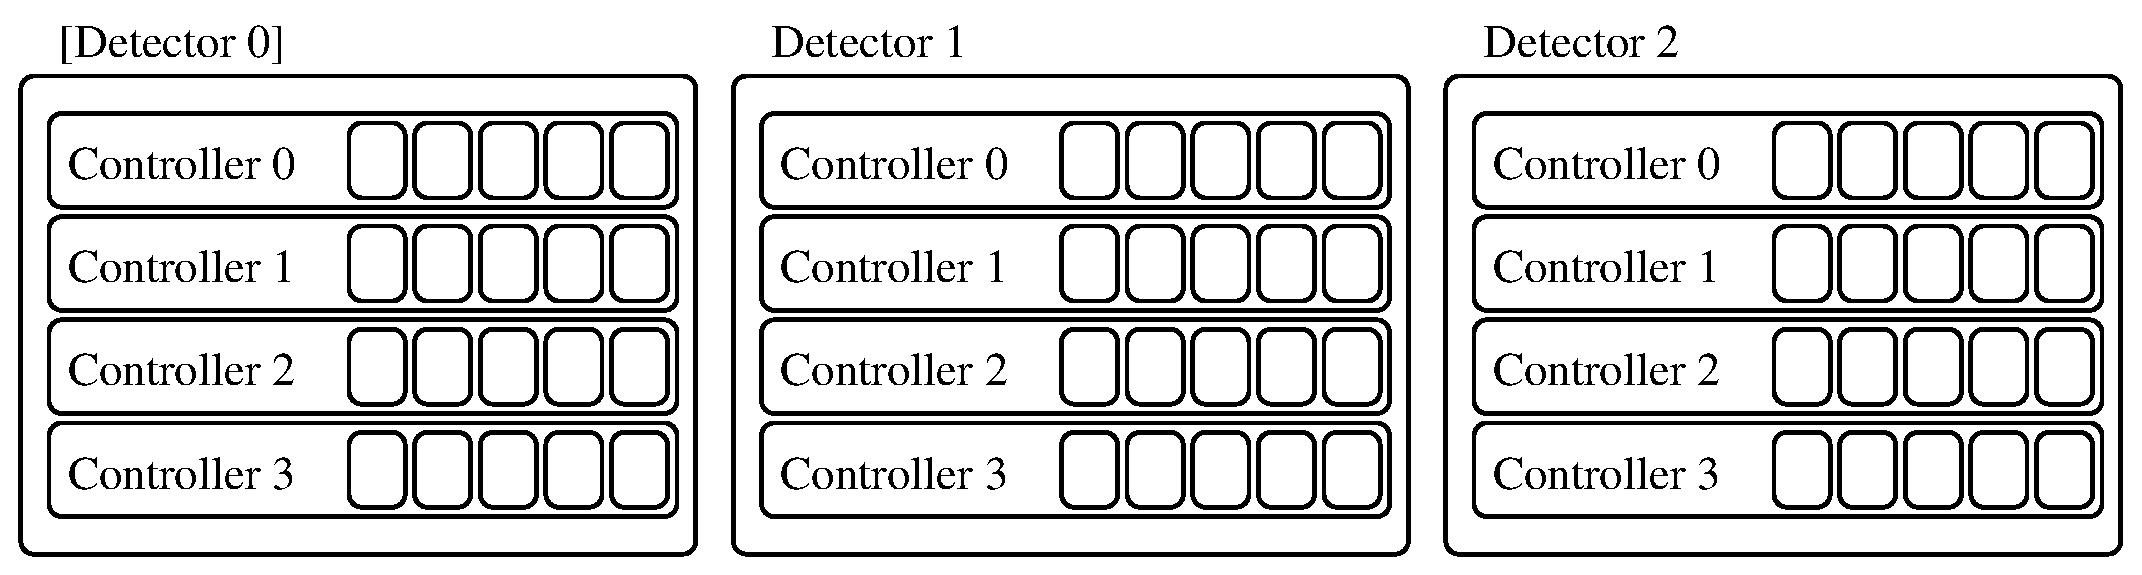
\includegraphics[width=\textwidth]{multi_detector}%
\lthtmlpictureZ
\lthtmlcheckvsize\clearpage}

\stepcounter{subsection}
\stepcounter{section}
{\newpage\clearpage
\lthtmlpictureA{tex2html_wrap2627}%
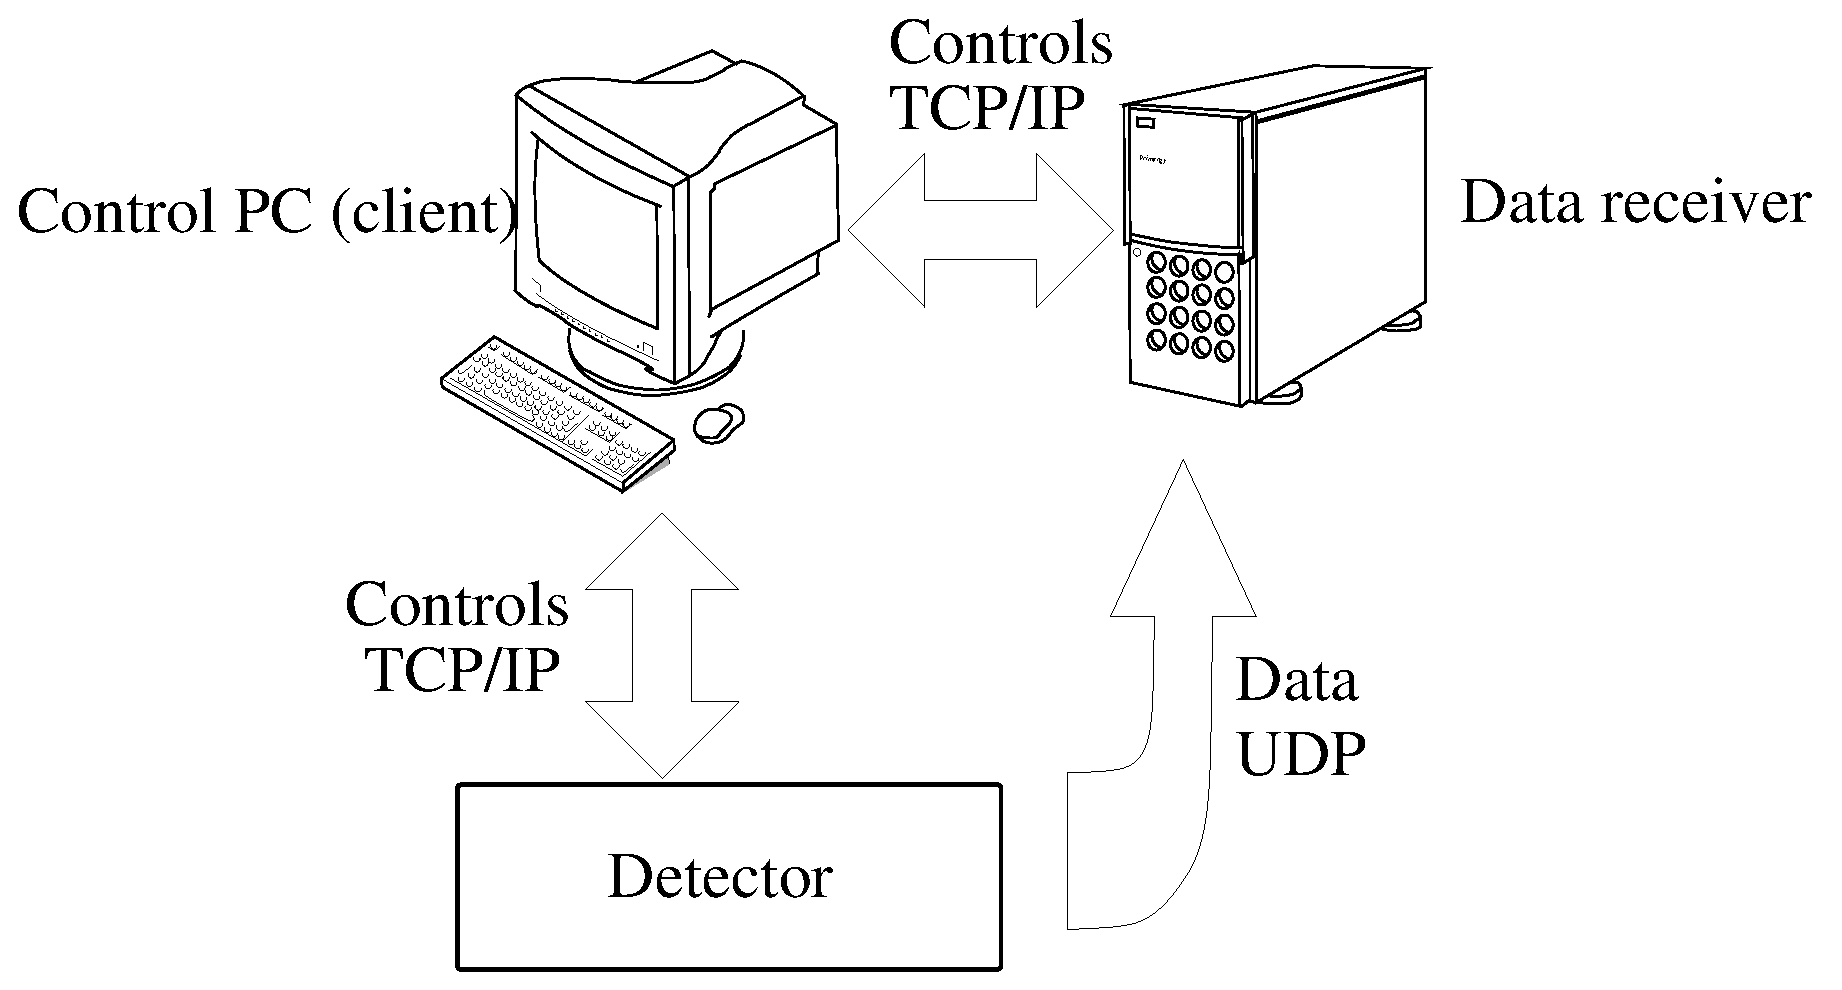
\includegraphics[width=\textwidth]{data_receiver}%
\lthtmlpictureZ
\lthtmlcheckvsize\clearpage}

\stepcounter{section}
\stepcounter{subsection}
\stepcounter{subsection}
\stepcounter{section}
\stepcounter{section}
{\newpage\clearpage
\lthtmlinlinemathA{tex2html_wrap_inline2637}%
$ d$%
\lthtmlinlinemathZ
\lthtmlcheckvsize\clearpage}

\stepcounter{section}
{\newpage\clearpage
\lthtmlinlinemathA{tex2html_wrap_inline2640}%
$ \Updownarrow$%
\lthtmlinlinemathZ
\lthtmlcheckvsize\clearpage}

{\newpage\clearpage
\lthtmlinlinemathA{tex2html_wrap_inline2642}%
$ \Rightarrow$%
\lthtmlinlinemathZ
\lthtmlcheckvsize\clearpage}

{\newpage\clearpage
\lthtmldisplayA{displaymath2644}%
\begin{displaymath}\textrm{\textbf{MEASUREMENTS}} \\
 \left\Updownarrow \,
    \begin{array}{l} \\
  %   \textrm{Measurement loop} \\
  \begin{array}{l} %\\
        	  \Rightarrow  \,  \textrm{Start script} \\
	   \\
\textrm{\textbf{SCAN0}}
           \left\Updownarrow 
     \,
	          \begin{array}{l} \\
                 	  \Rightarrow \,  \textrm{Scan0 script} \\
           %        \textrm{Scan 0 level} \\
		   \\
\par
\textrm{\textbf{SCAN1}}      \left\Updownarrow  
     \,
	          \begin{array}{l} \\
                %   \textrm{Scan 1 level} \\
		 \begin{array}{l} %\\
                 	  \Rightarrow \,  \textrm{Scan1 script} \\
                 	  \Rightarrow \,  \textrm{Script before} \\
		   \\
\begin{array}{l} \\
                    \textrm{\textbf{POSITIONS}} \left\Updownarrow  \,	  
\begin{array}{l} \\
             	  \Rightarrow \,     \textrm{Header before script} \\
		   \\
\par
\textrm{\textbf{CYCLES}}     \left\Updownarrow  \,
	          \begin{array}{l} \\
		  \\
\textrm{\textbf{FRAMES}}    \left\Updownarrow  \right. \\
		  \\
\\
		  \end{array}
		  \right. \\
		  \\
\Rightarrow \,  \textrm{Header after script}\\
		  \\
		  \end{array}
		  \right. \\
\\
\\
\\
           \end{array}
\par
\\
	 %  \\
\Rightarrow \, \textrm{Script after} \\
\end{array}
	  % \right. \\
	   \\
\\
                   \end{array}
	   \right. \\
\\
	   \\
\\
                   \end{array} 
	   \right. \\
	   \\
\Rightarrow	\,   \textrm{Stop script} \\
\\
            \end{array} 
 %     \right. \\
 \\
      \end{array}  
\right. 
\end{displaymath}%
\lthtmldisplayZ
\lthtmlcheckvsize\clearpage}

\stepcounter{section}
{\newpage\clearpage
\lthtmlpictureA{tex2html_wrap2667}%
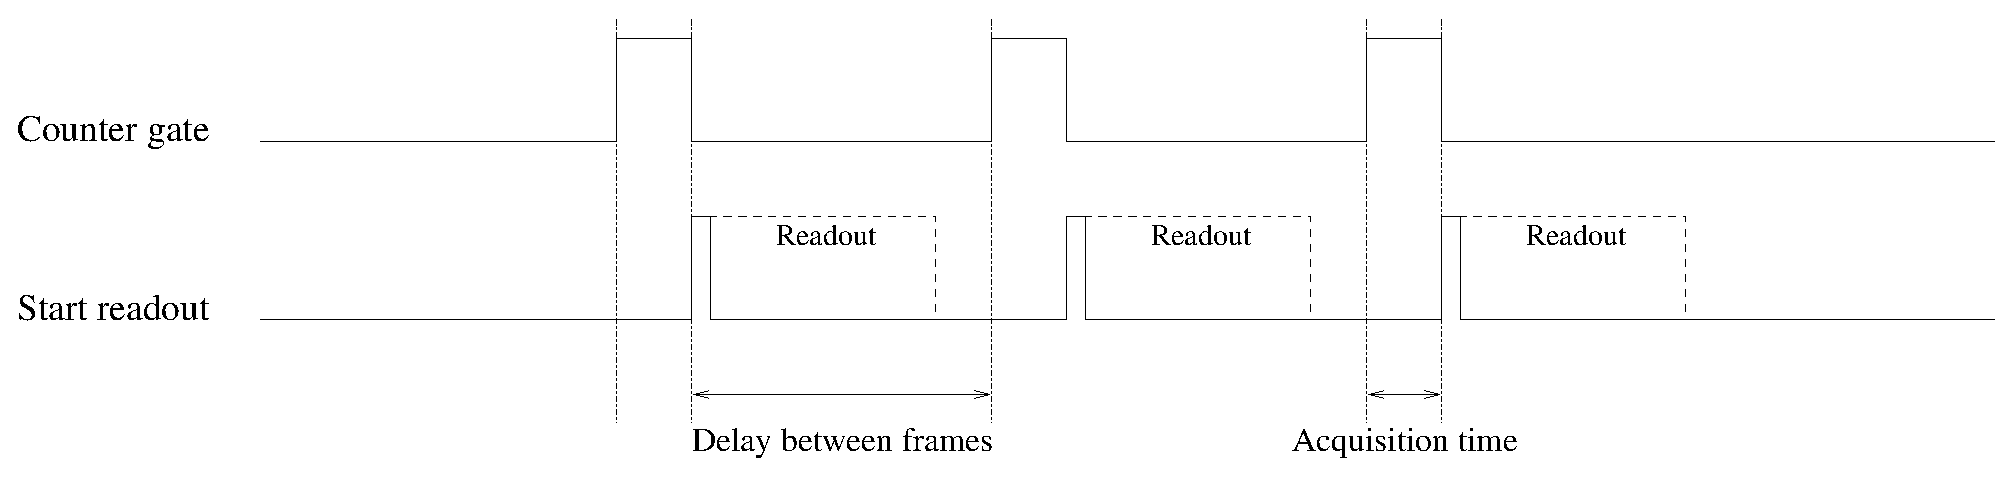
\includegraphics[width=\textwidth]{images/normal_acquisition.eps}%
\lthtmlpictureZ
\lthtmlcheckvsize\clearpage}

{\newpage\clearpage
\lthtmlpictureA{tex2html_wrap2671}%
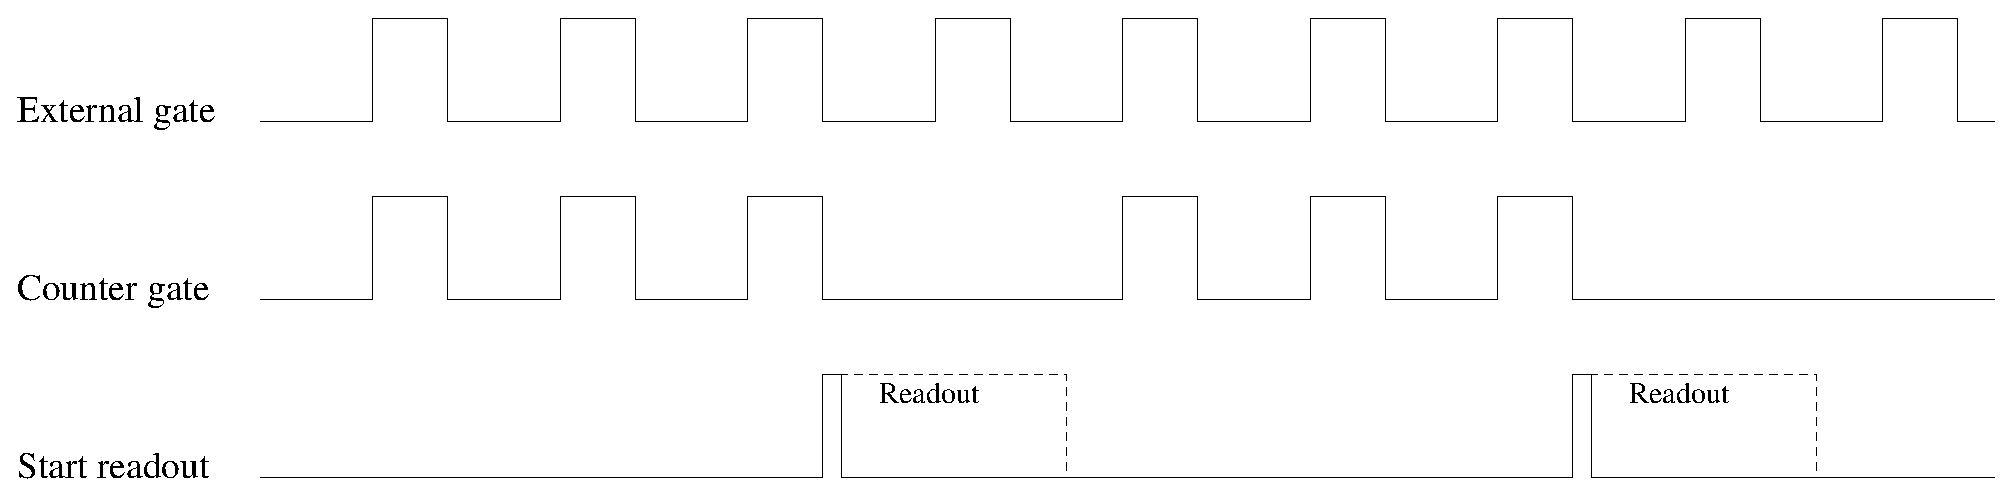
\includegraphics[width=\textwidth]{images/gated_acquisition.eps}%
\lthtmlpictureZ
\lthtmlcheckvsize\clearpage}

{\newpage\clearpage
\lthtmlpictureA{tex2html_wrap2675}%
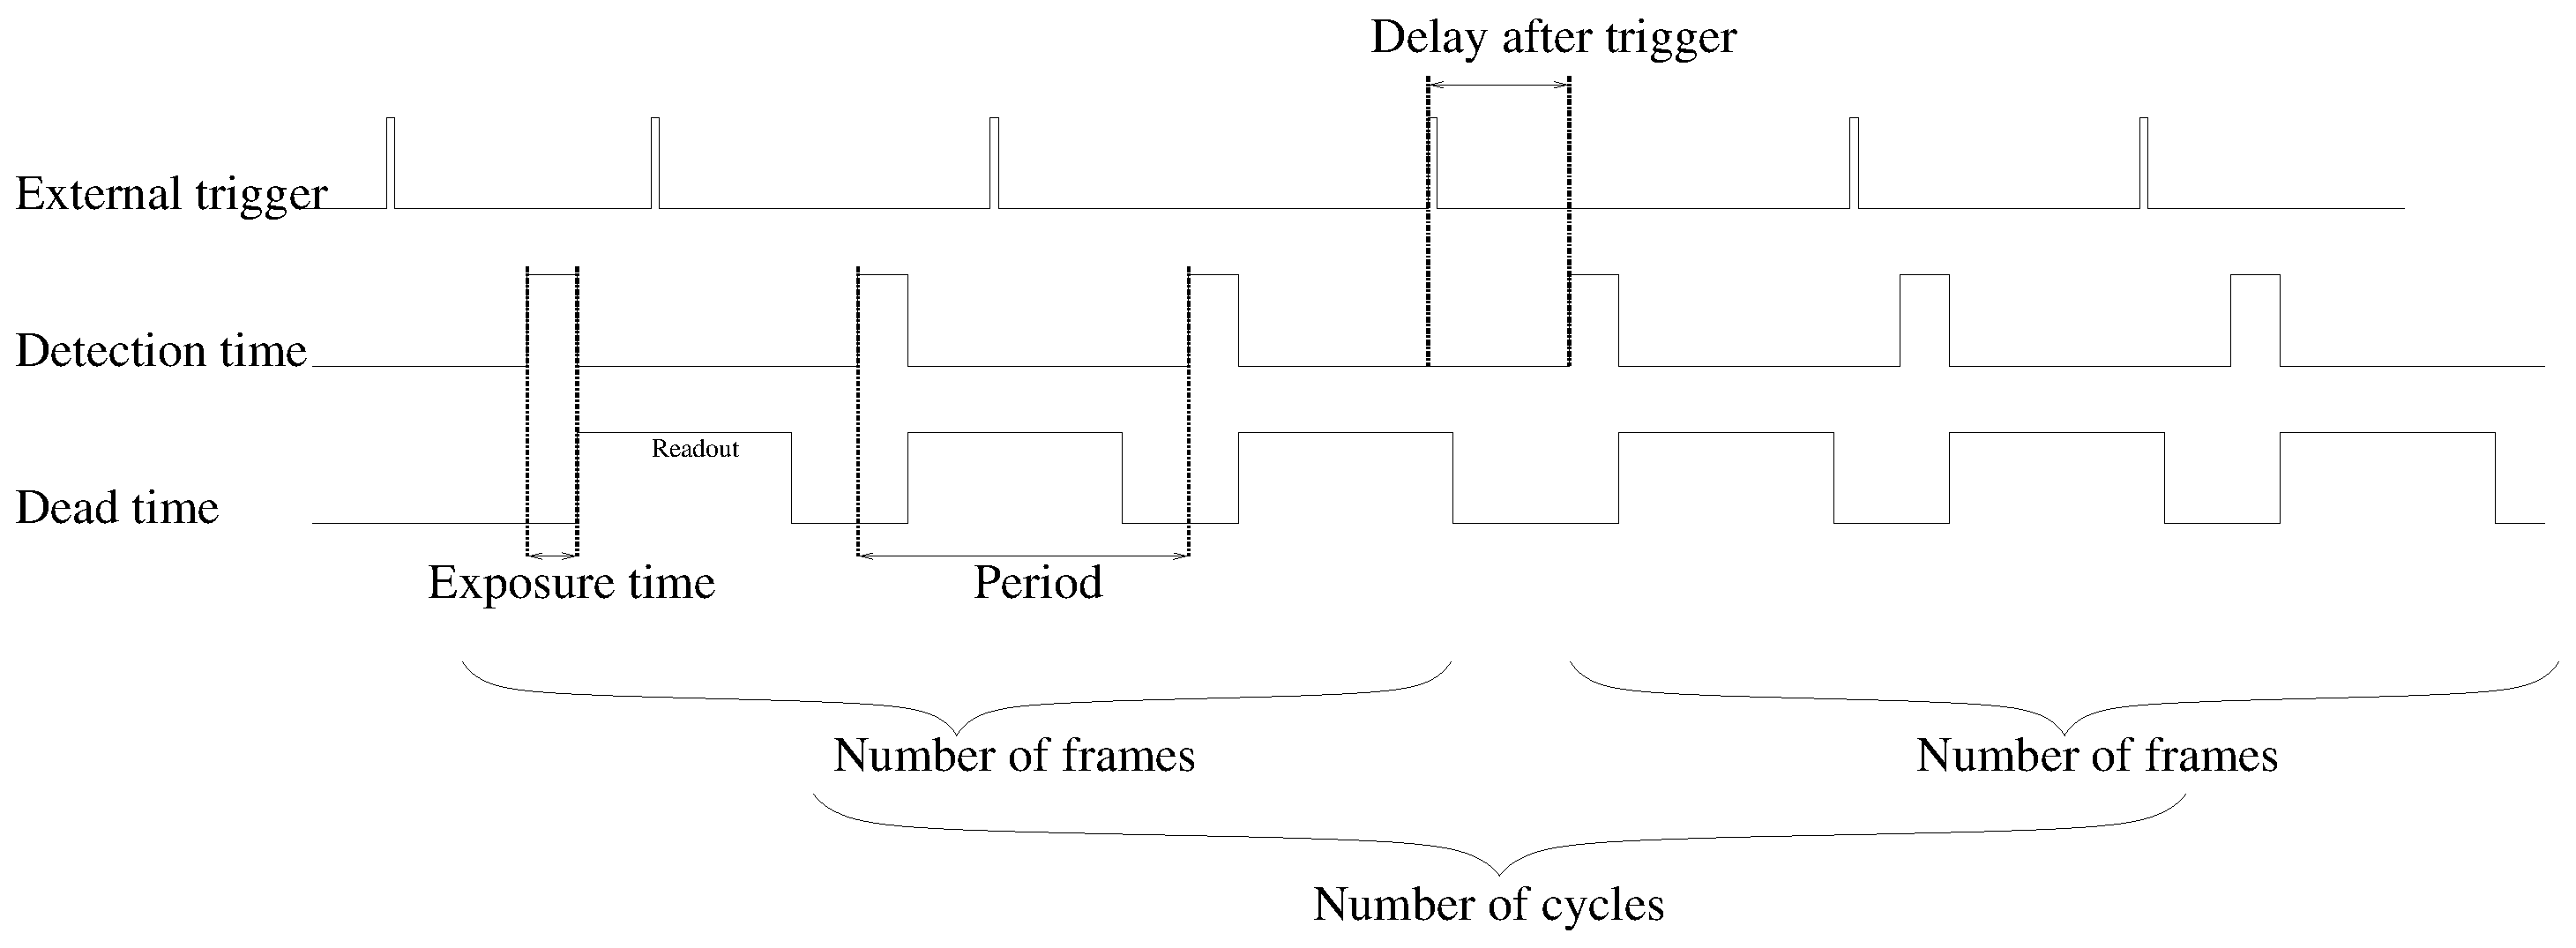
\includegraphics[width=\textwidth]{images/trigger_acquisition.eps}%
\lthtmlpictureZ
\lthtmlcheckvsize\clearpage}

{\newpage\clearpage
\lthtmlpictureA{tex2html_wrap2679}%
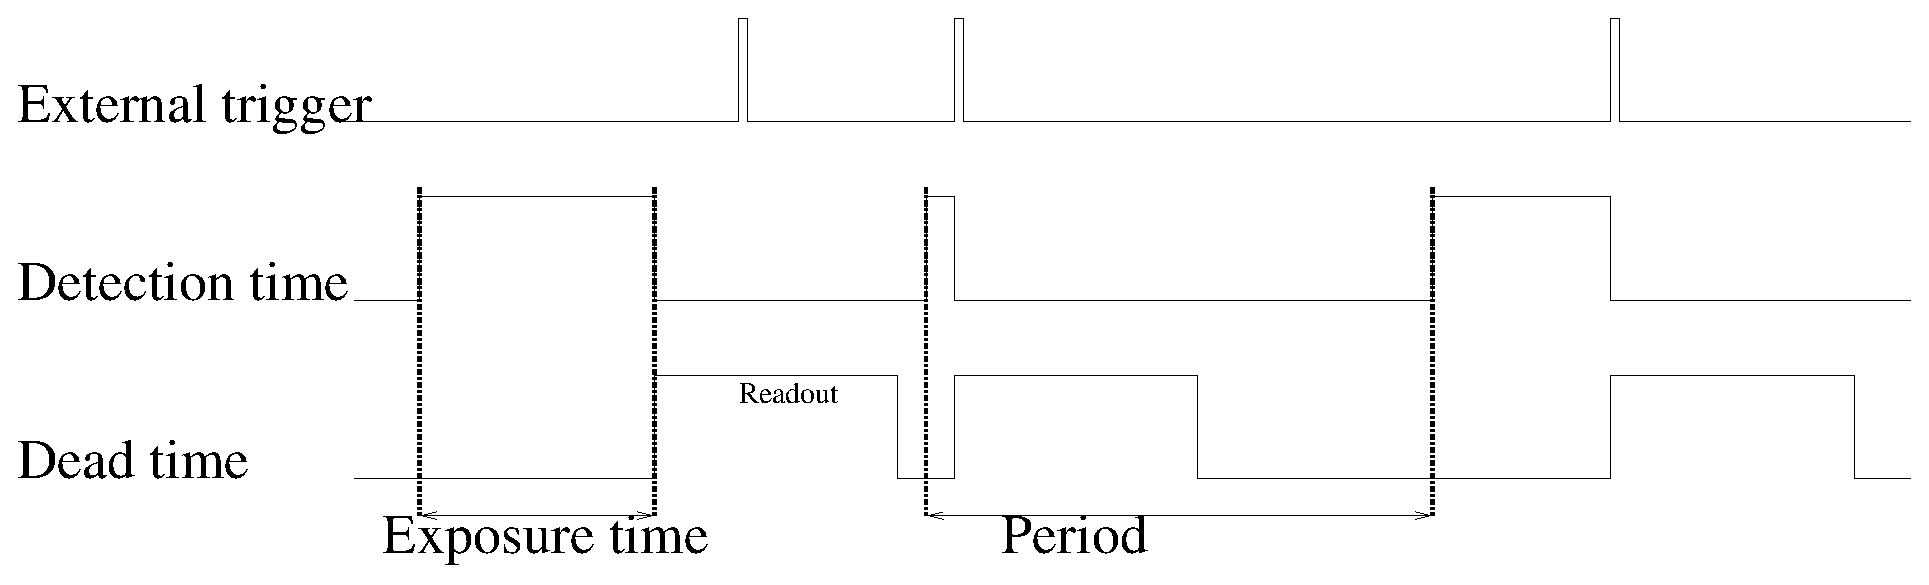
\includegraphics[width=\textwidth]{images/ro_trigger_acquisition.eps}%
\lthtmlpictureZ
\lthtmlcheckvsize\clearpage}

\stepcounter{section}
\stepcounter{section}
\stepcounter{section}
\stepcounter{subsection}
{\newpage\clearpage
\lthtmlinlinemathA{tex2html_wrap_inline2690}%
$ (108602\&0xFFFFFFFE)>>1 = 54301$%
\lthtmlinlinemathZ
\lthtmlcheckvsize\clearpage}

{\newpage\clearpage
\lthtmlinlinemathA{tex2html_wrap_inline2692}%
$ (108602\&0x1) =0$%
\lthtmlinlinemathZ
\lthtmlcheckvsize\clearpage}

\stepcounter{subsection}
\stepcounter{subsection}
\stepcounter{chapter}
\stepcounter{section}
\stepcounter{subsection}
{\newpage\clearpage
\lthtmlpictureA{tex2html_wrap2698}%
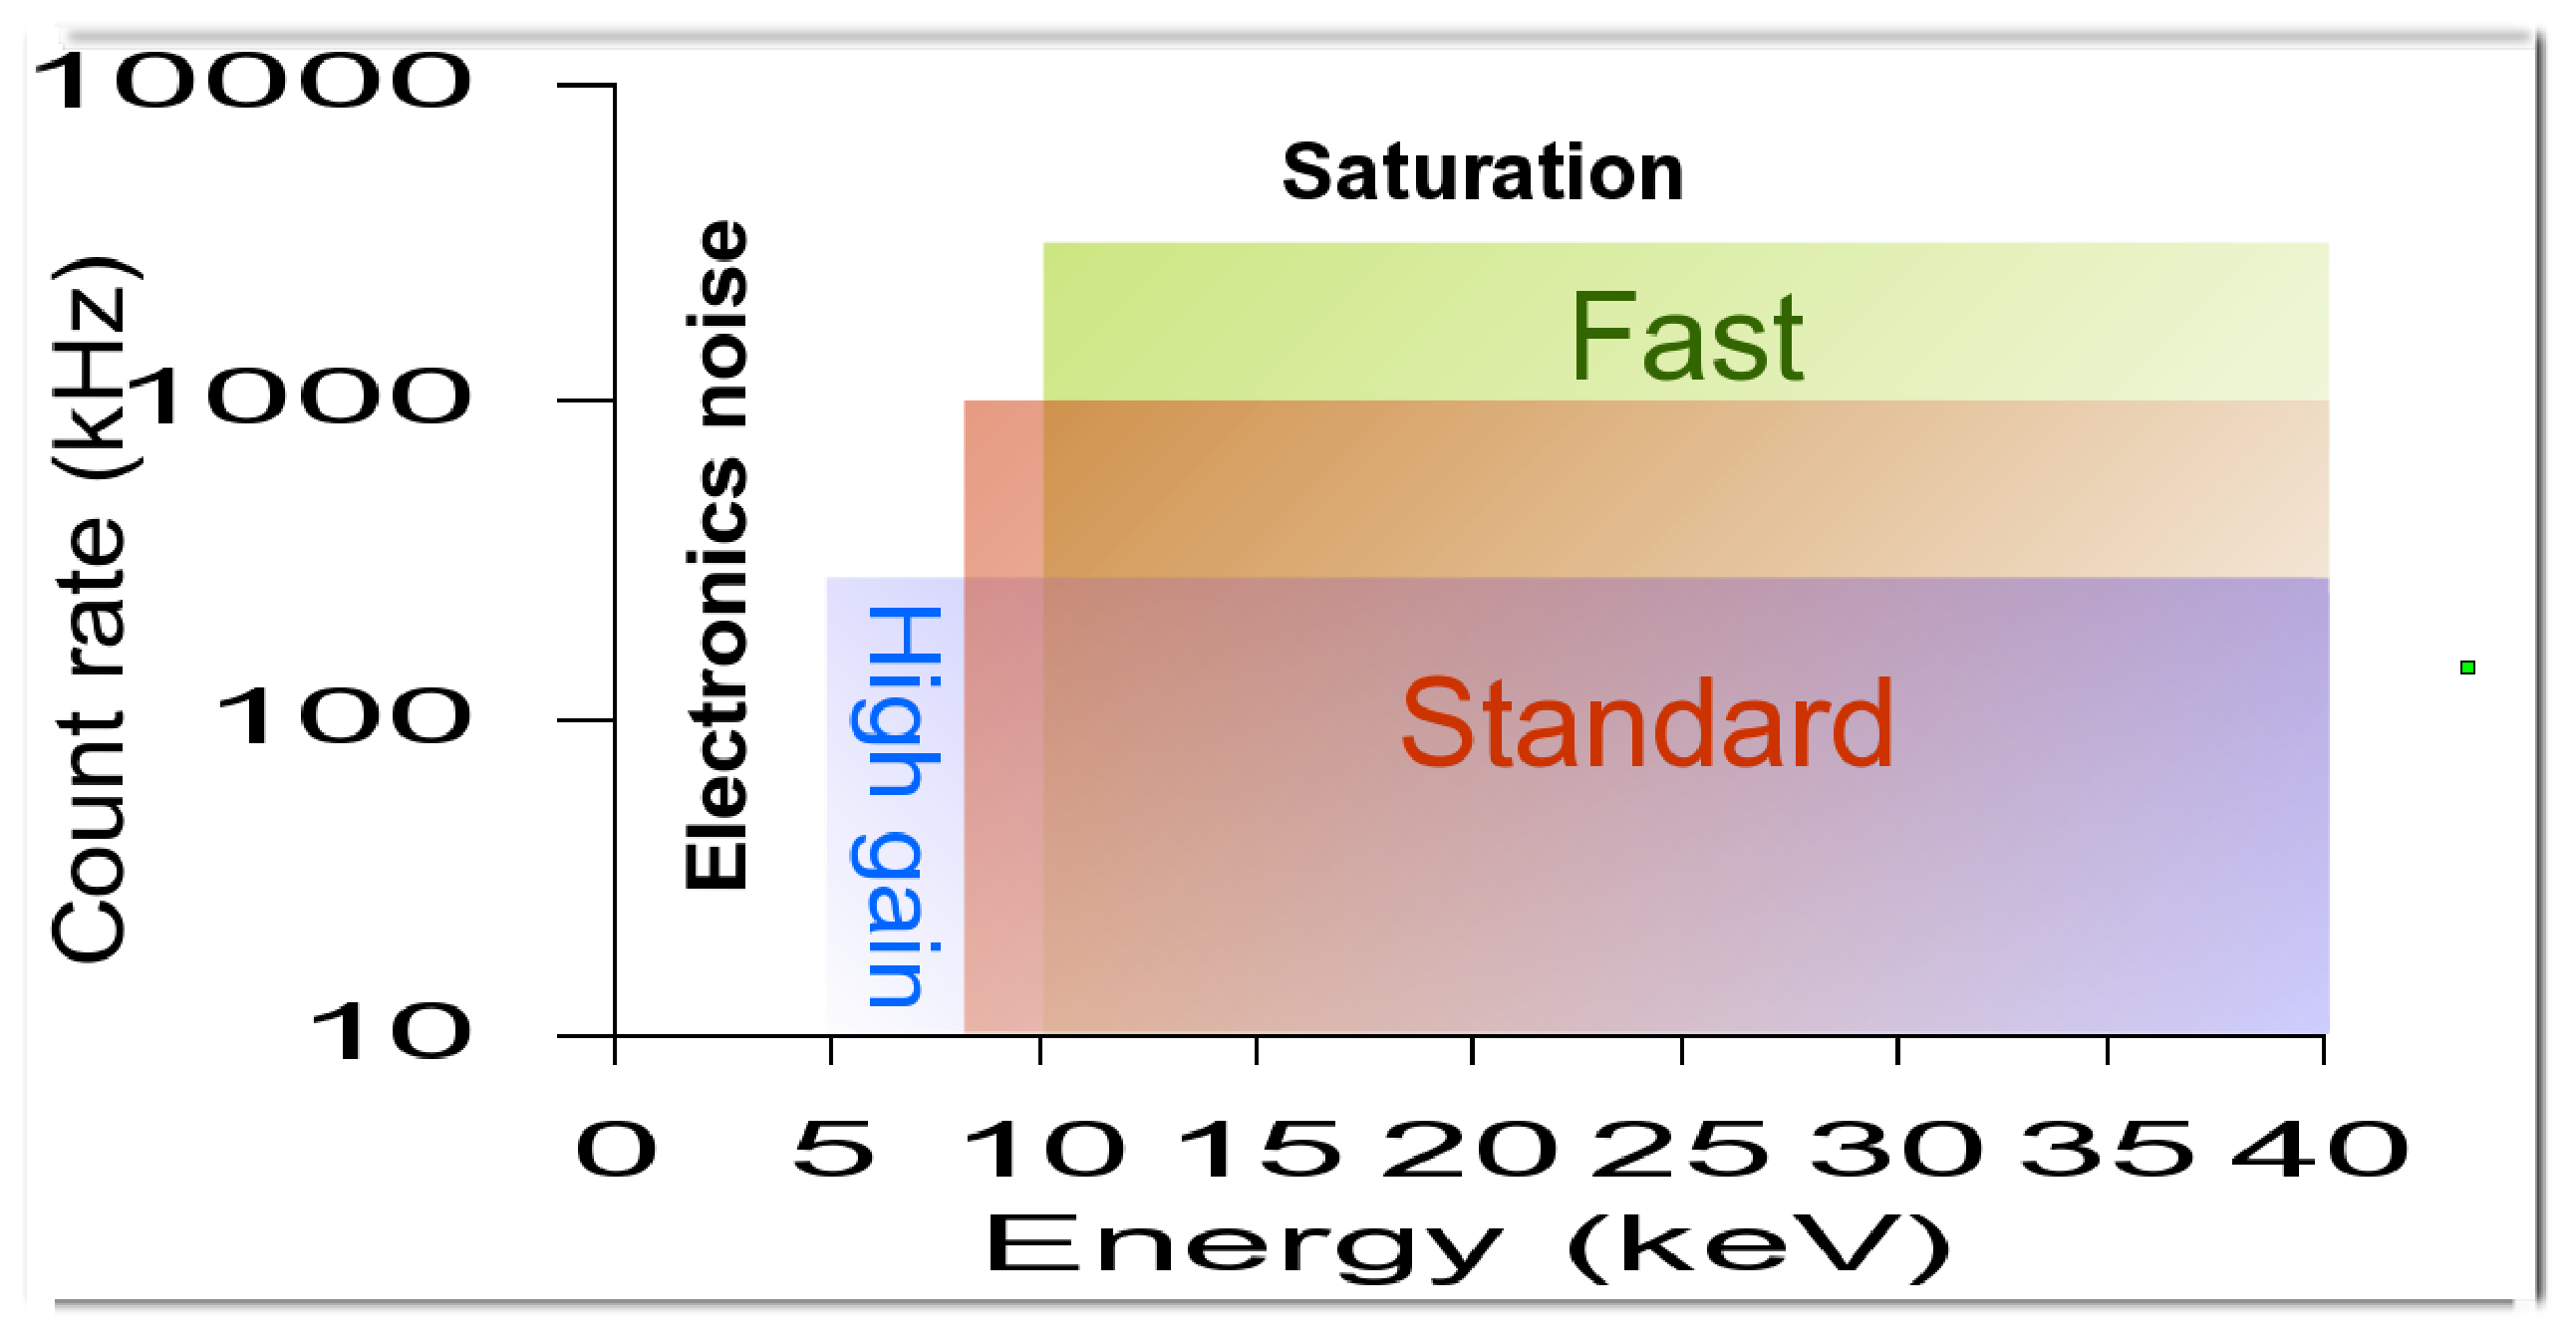
\includegraphics[width=\textwidth]{images/settings}%
\lthtmlpictureZ
\lthtmlcheckvsize\clearpage}

\stepcounter{section}
{\newpage\clearpage
\lthtmlpictureA{tex2html_wrap2703}%
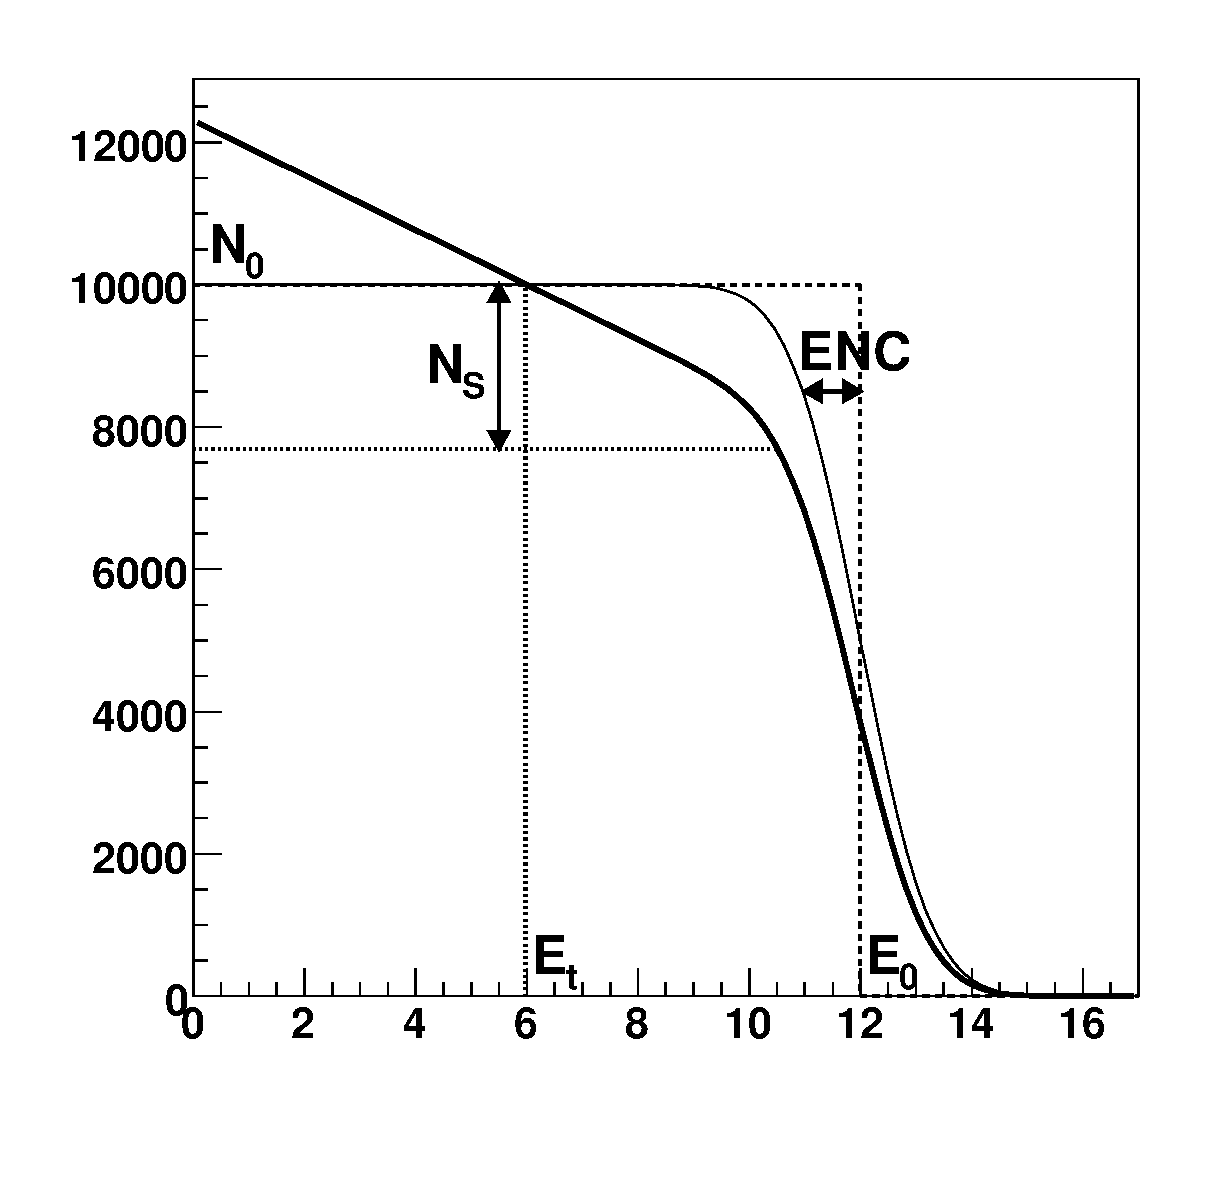
\includegraphics[width=\textwidth]{images/thr_scan_expl}%
\lthtmlpictureZ
\lthtmlcheckvsize\clearpage}

{\newpage\clearpage
\lthtmlpictureA{tex2html_wrap2707}%
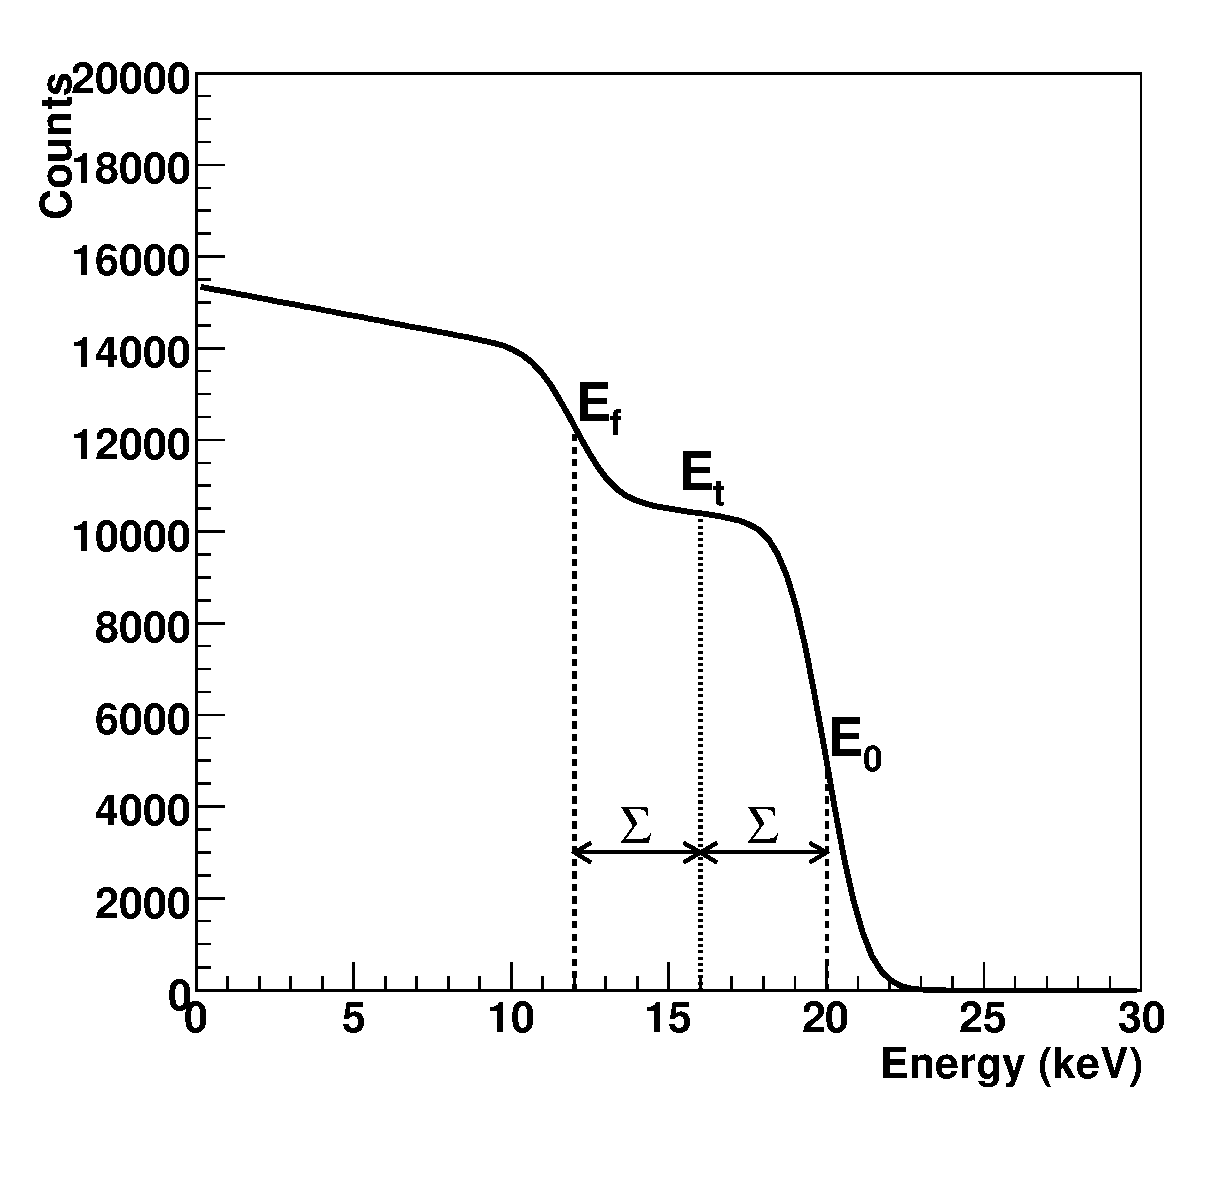
\includegraphics[width=\textwidth]{images/thr_scan_fluo}%
\lthtmlpictureZ
\lthtmlcheckvsize\clearpage}

{\newpage\clearpage
\lthtmlinlinemathA{tex2html_wrap_inline2712}%
$ E_0$%
\lthtmlinlinemathZ
\lthtmlcheckvsize\clearpage}

{\newpage\clearpage
\lthtmlinlinemathA{tex2html_wrap_inline2716}%
$ E_t=E_0/2$%
\lthtmlinlinemathZ
\lthtmlcheckvsize\clearpage}

{\newpage\clearpage
\lthtmlinlinemathA{tex2html_wrap_inline2720}%
$ E_f$%
\lthtmlinlinemathZ
\lthtmlcheckvsize\clearpage}

{\newpage\clearpage
\lthtmlinlinemathA{tex2html_wrap_inline2724}%
$ E_t$%
\lthtmlinlinemathZ
\lthtmlcheckvsize\clearpage}

{\newpage\clearpage
\lthtmlinlinemathA{tex2html_wrap_inline2738}%
$ E_f<E_0$%
\lthtmlinlinemathZ
\lthtmlcheckvsize\clearpage}

{\newpage\clearpage
\lthtmlinlinemathA{tex2html_wrap_inline2742}%
$ E_t>E_f+3$%
\lthtmlinlinemathZ
\lthtmlcheckvsize\clearpage}

{\newpage\clearpage
\lthtmlinlinemathA{tex2html_wrap_inline2744}%
$ E_t<E_0-3$%
\lthtmlinlinemathZ
\lthtmlcheckvsize\clearpage}

{\newpage\clearpage
\lthtmlinlinemathA{tex2html_wrap_inline2756}%
$ E_t<E_f-3$%
\lthtmlinlinemathZ
\lthtmlcheckvsize\clearpage}

{\newpage\clearpage
\lthtmlinlinemathA{tex2html_wrap_inline2760}%
$ E_t>4$%
\lthtmlinlinemathZ
\lthtmlcheckvsize\clearpage}

{\newpage\clearpage
\lthtmlpictureA{tex2html_wrap2767}%
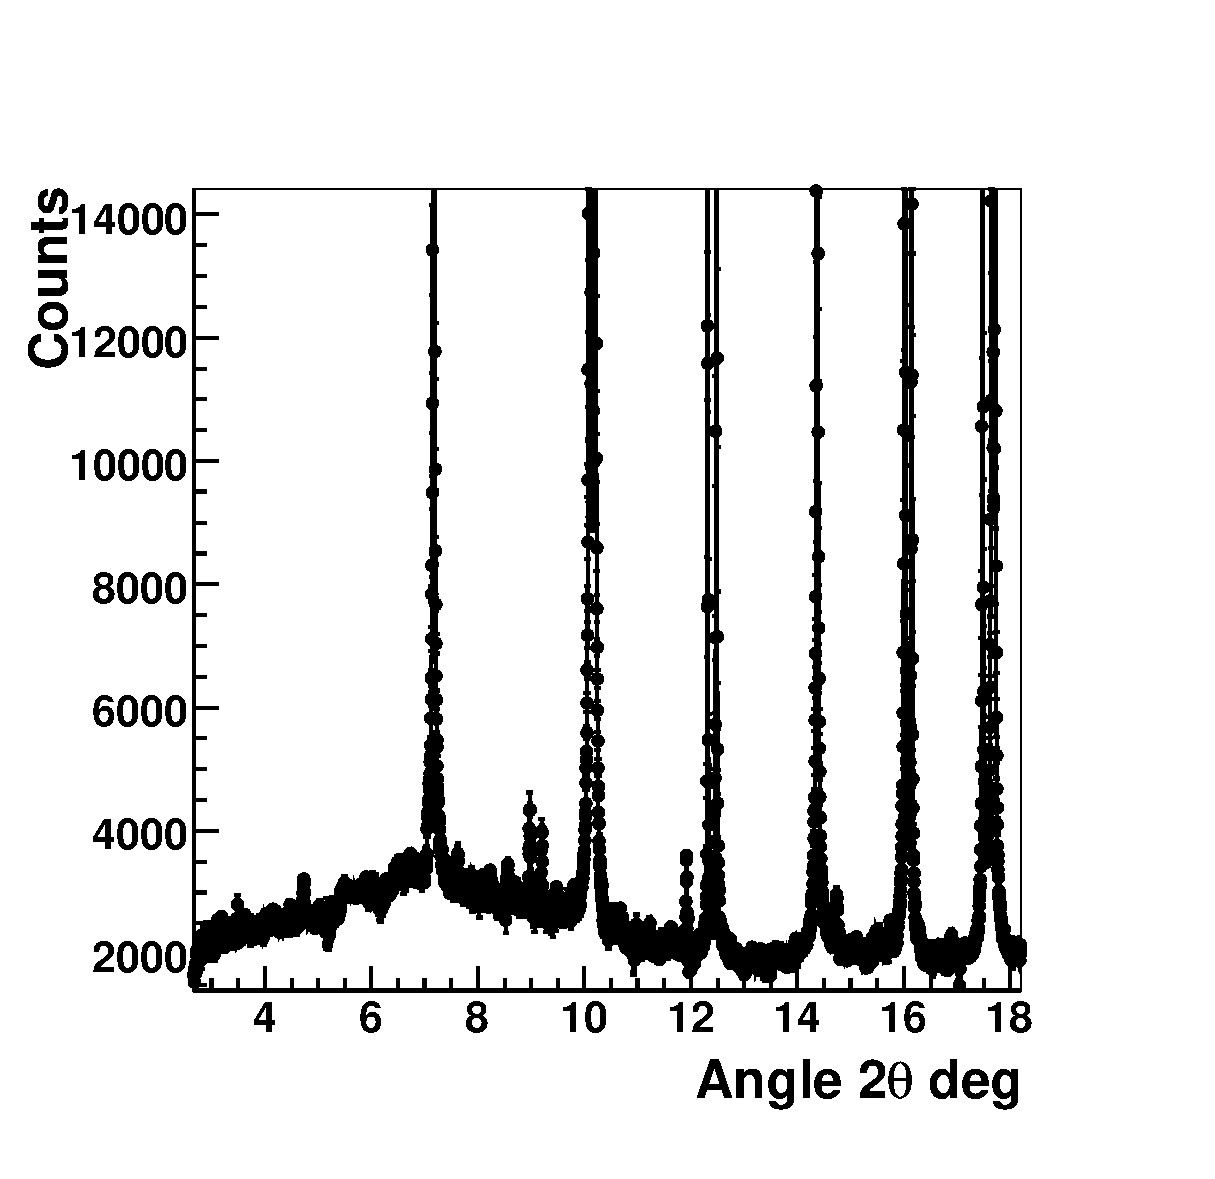
\includegraphics[width=\textwidth]{images/sample_with_fluorescence}%
\lthtmlpictureZ
\lthtmlcheckvsize\clearpage}

\stepcounter{section}
\stepcounter{subsection}
{\newpage\clearpage
\lthtmlpictureA{tex2html_wrap2773}%
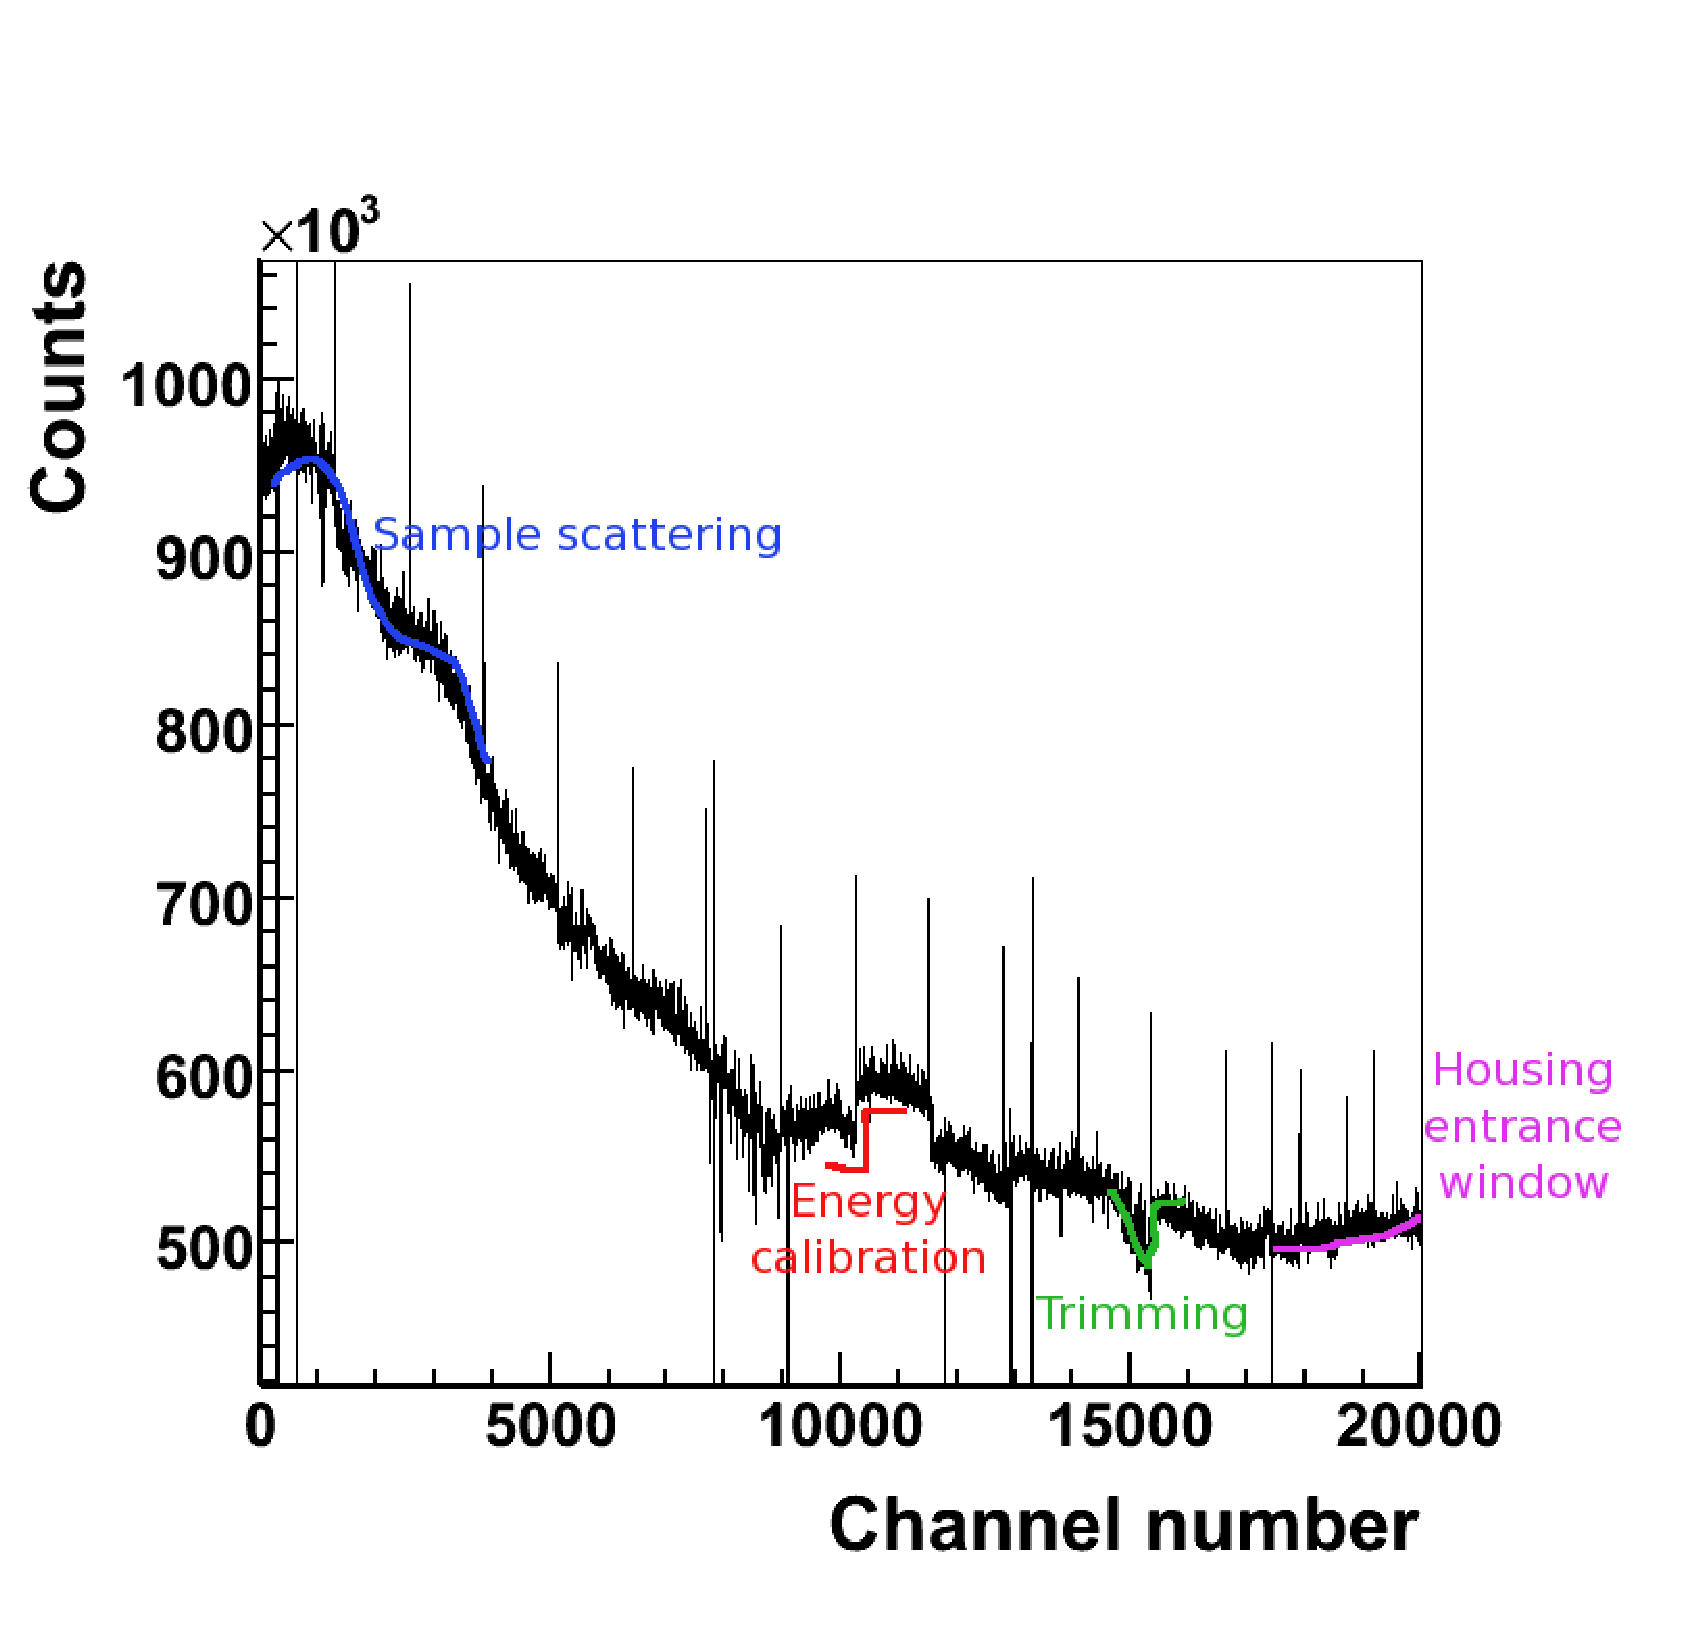
\includegraphics[width=\textwidth]{images/bad_ff_col}%
\lthtmlpictureZ
\lthtmlcheckvsize\clearpage}

\stepcounter{subsection}
{\newpage\clearpage
\lthtmlpictureA{tex2html_wrap2778}%
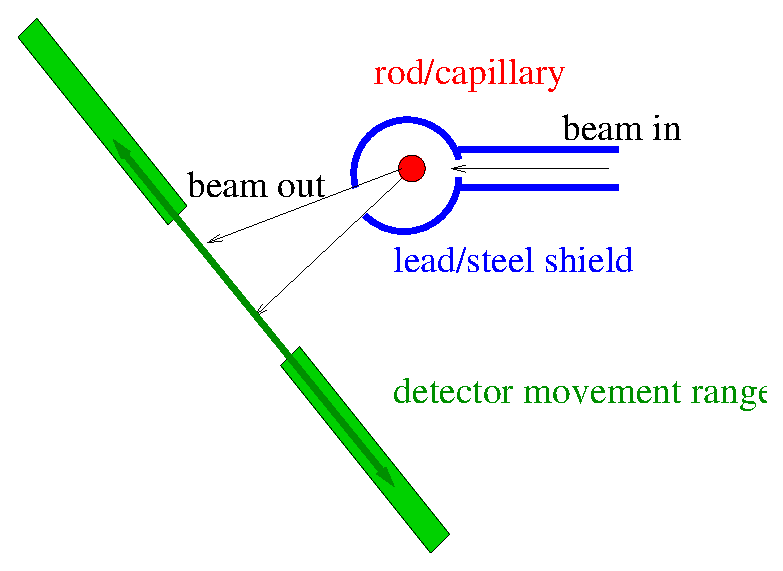
\includegraphics[width=\textwidth]{images/FFSetup}%
\lthtmlpictureZ
\lthtmlcheckvsize\clearpage}

\stepcounter{section}
\stepcounter{subsection}
{\newpage\clearpage
\lthtmlinlinemathA{tex2html_wrap_inline2785}%
$ Vthreshold=7$%
\lthtmlinlinemathZ
\lthtmlcheckvsize\clearpage}

{\newpage\clearpage
\lthtmlinlinemathA{tex2html_wrap_inline2787}%
$ Counts=500$%
\lthtmlinlinemathZ
\lthtmlcheckvsize\clearpage}

{\newpage\clearpage
\lthtmlinlinemathA{tex2html_wrap_inline2789}%
$ Resolution=4$%
\lthtmlinlinemathZ
\lthtmlcheckvsize\clearpage}

{\newpage\clearpage
\lthtmlinlinemathA{tex2html_wrap_inline2791}%
$ \pm$%
\lthtmlinlinemathZ
\lthtmlcheckvsize\clearpage}

{\newpage\clearpage
\lthtmlpictureA{tex2html_wrap2792}%
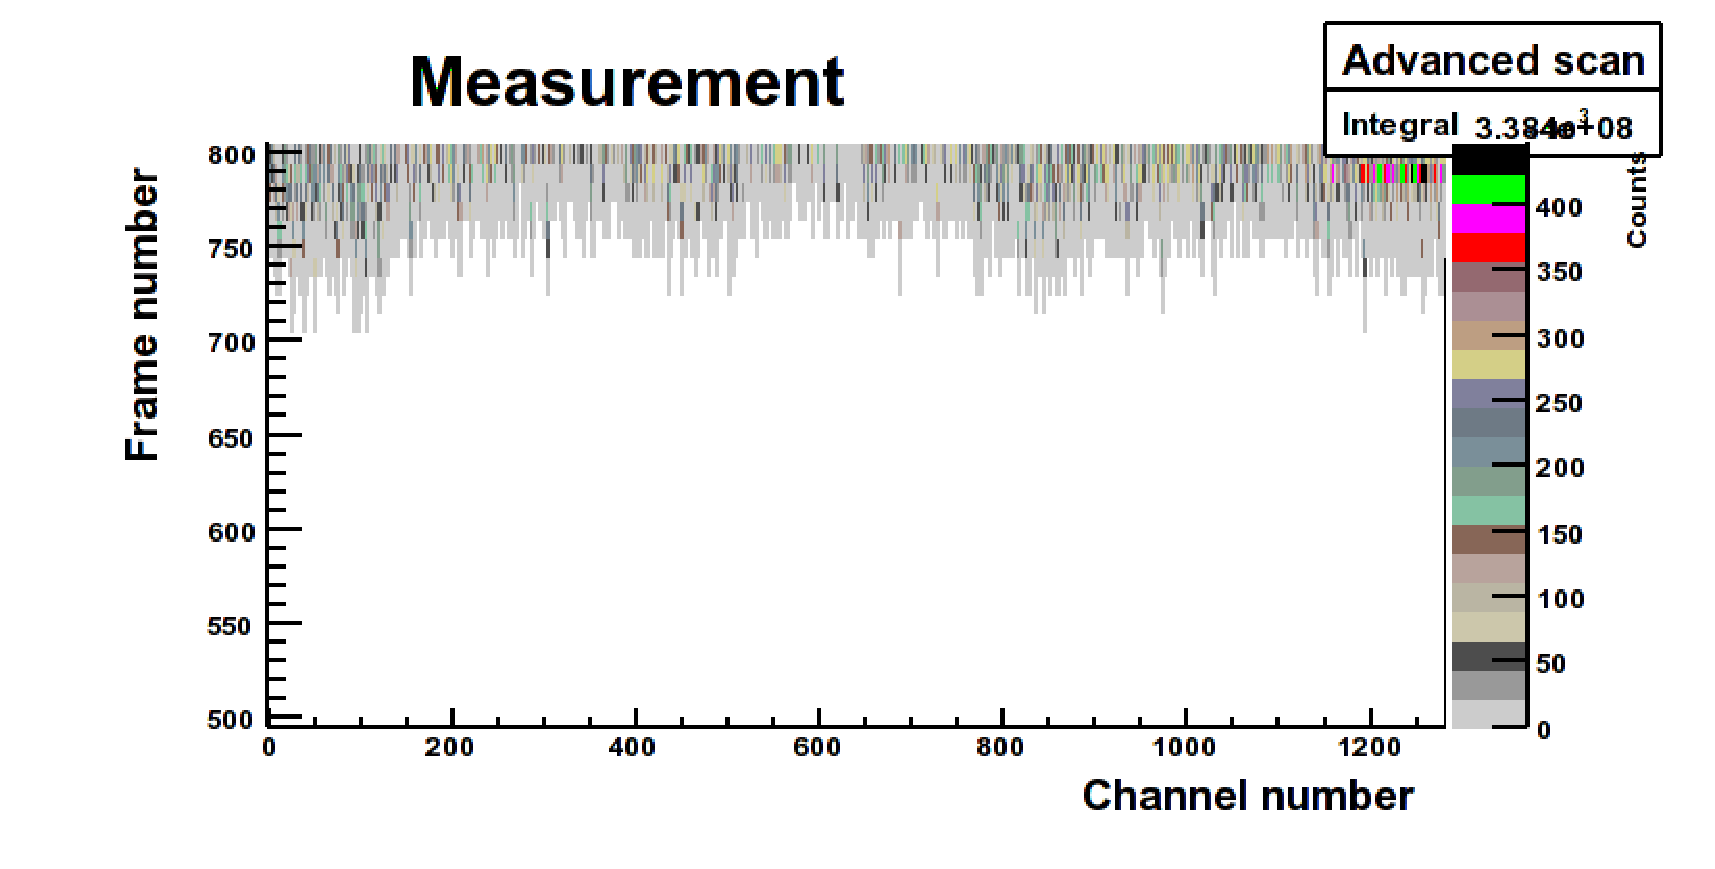
\includegraphics[width=\textwidth]{images/noise_thresholdscanuntrimmed}%
\lthtmlpictureZ
\lthtmlcheckvsize\clearpage}

{\newpage\clearpage
\lthtmlpictureA{tex2html_wrap2796}%
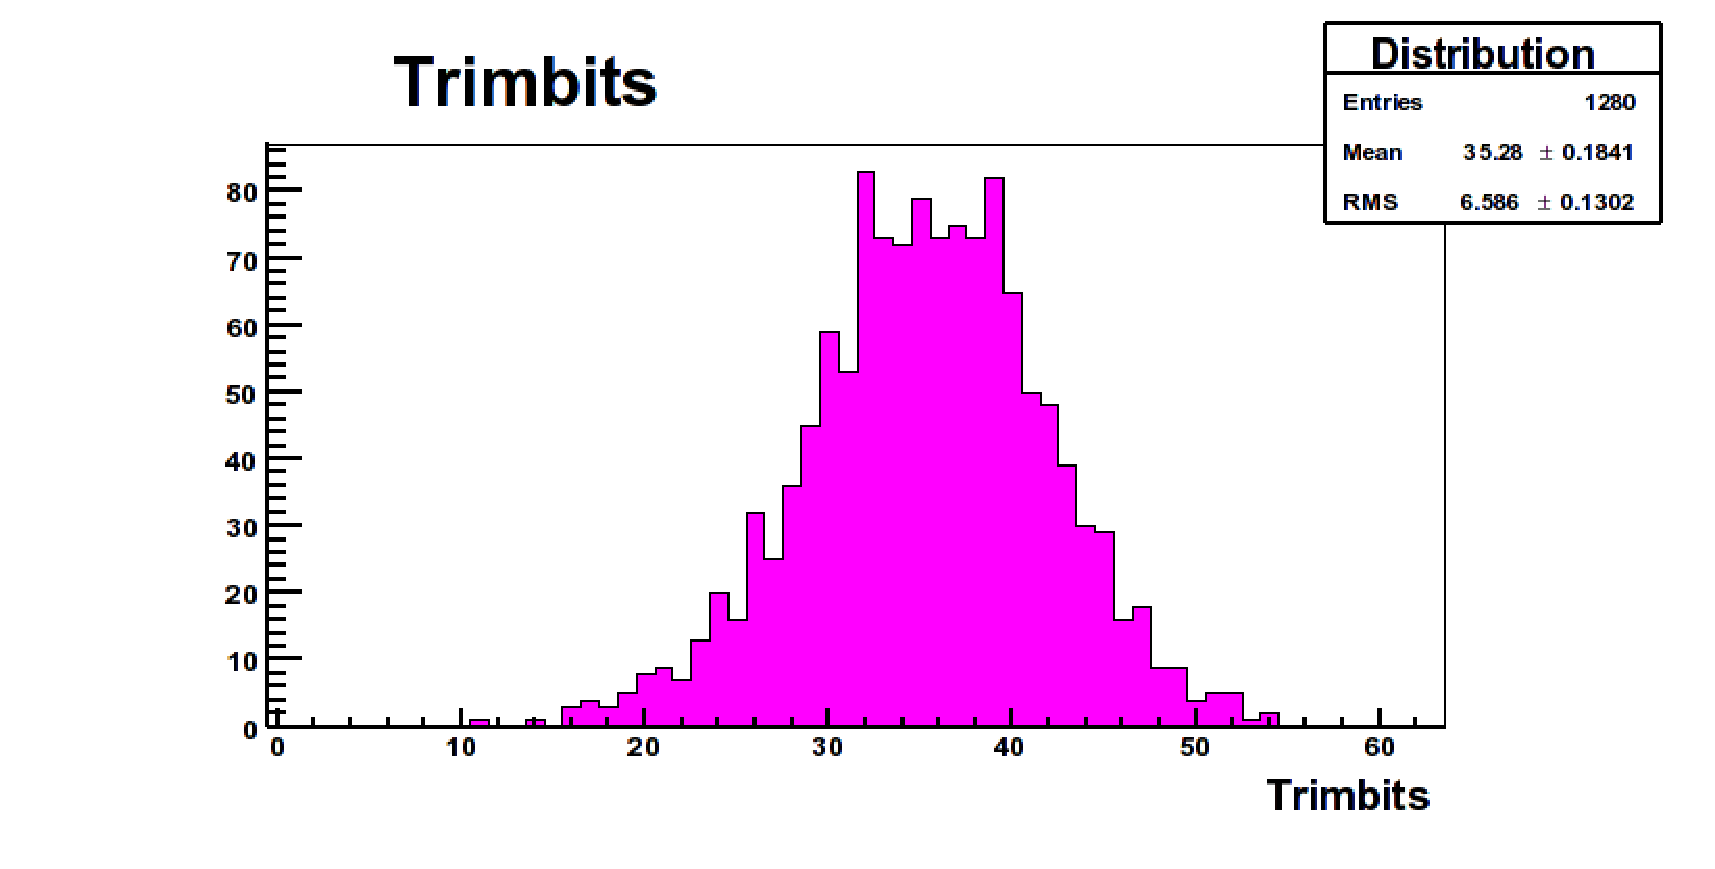
\includegraphics[width=\textwidth]{images/trimbitdistribution}%
\lthtmlpictureZ
\lthtmlcheckvsize\clearpage}

{\newpage\clearpage
\lthtmlpictureA{tex2html_wrap2800}%
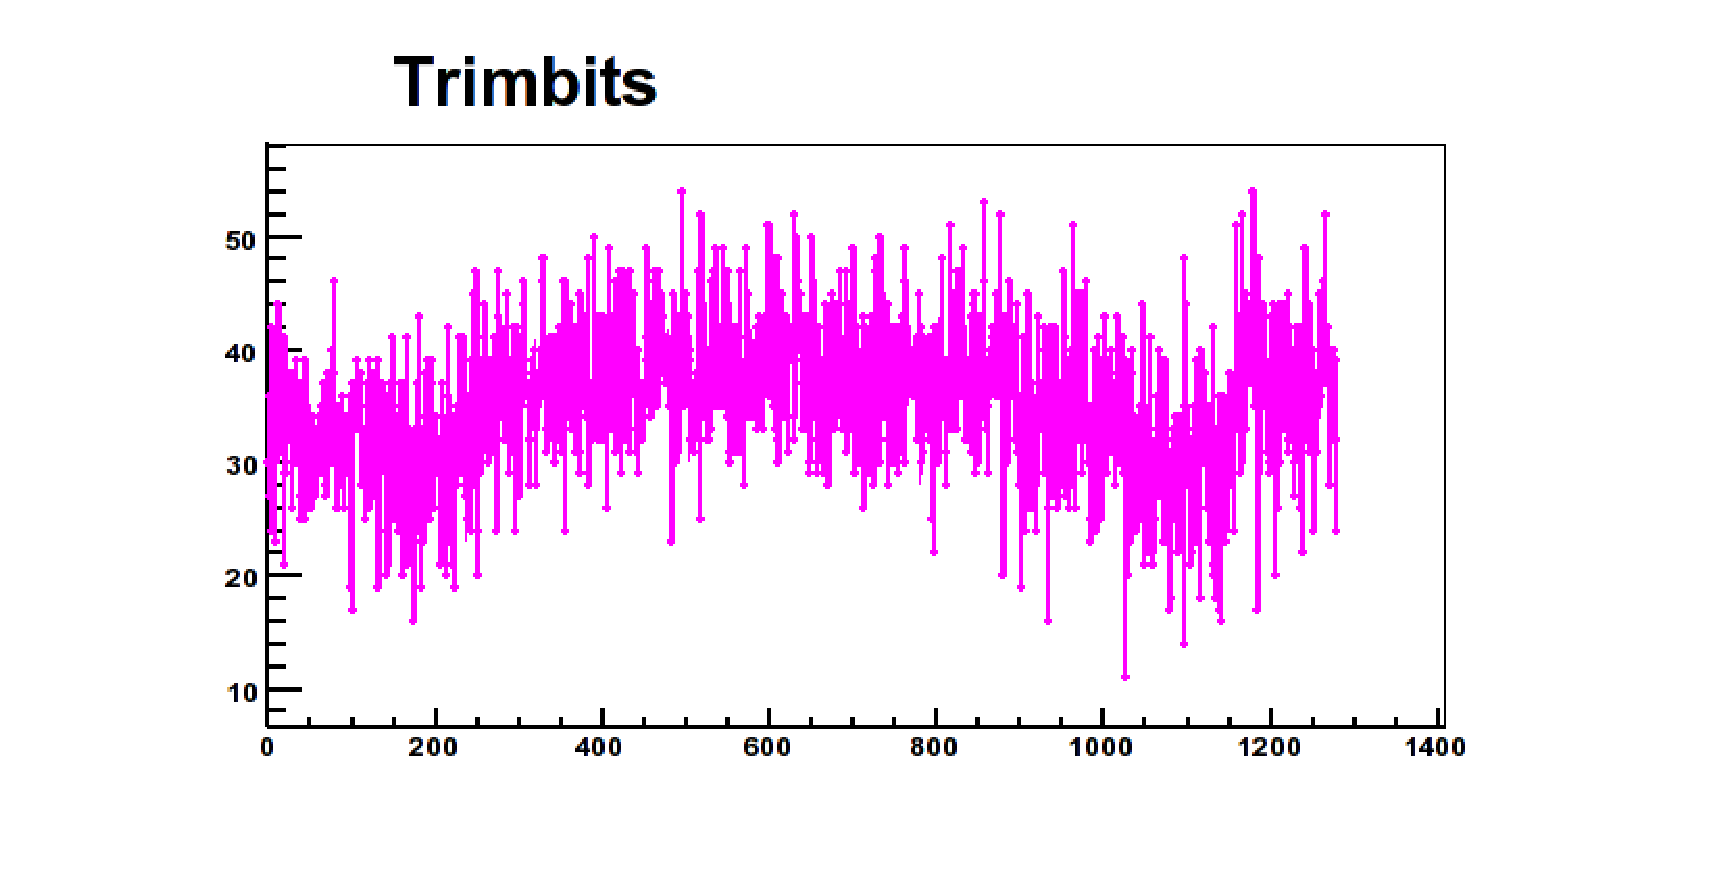
\includegraphics[width=\textwidth]{images/trimbitplot}%
\lthtmlpictureZ
\lthtmlcheckvsize\clearpage}

{\newpage\clearpage
\lthtmlpictureA{tex2html_wrap2804}%
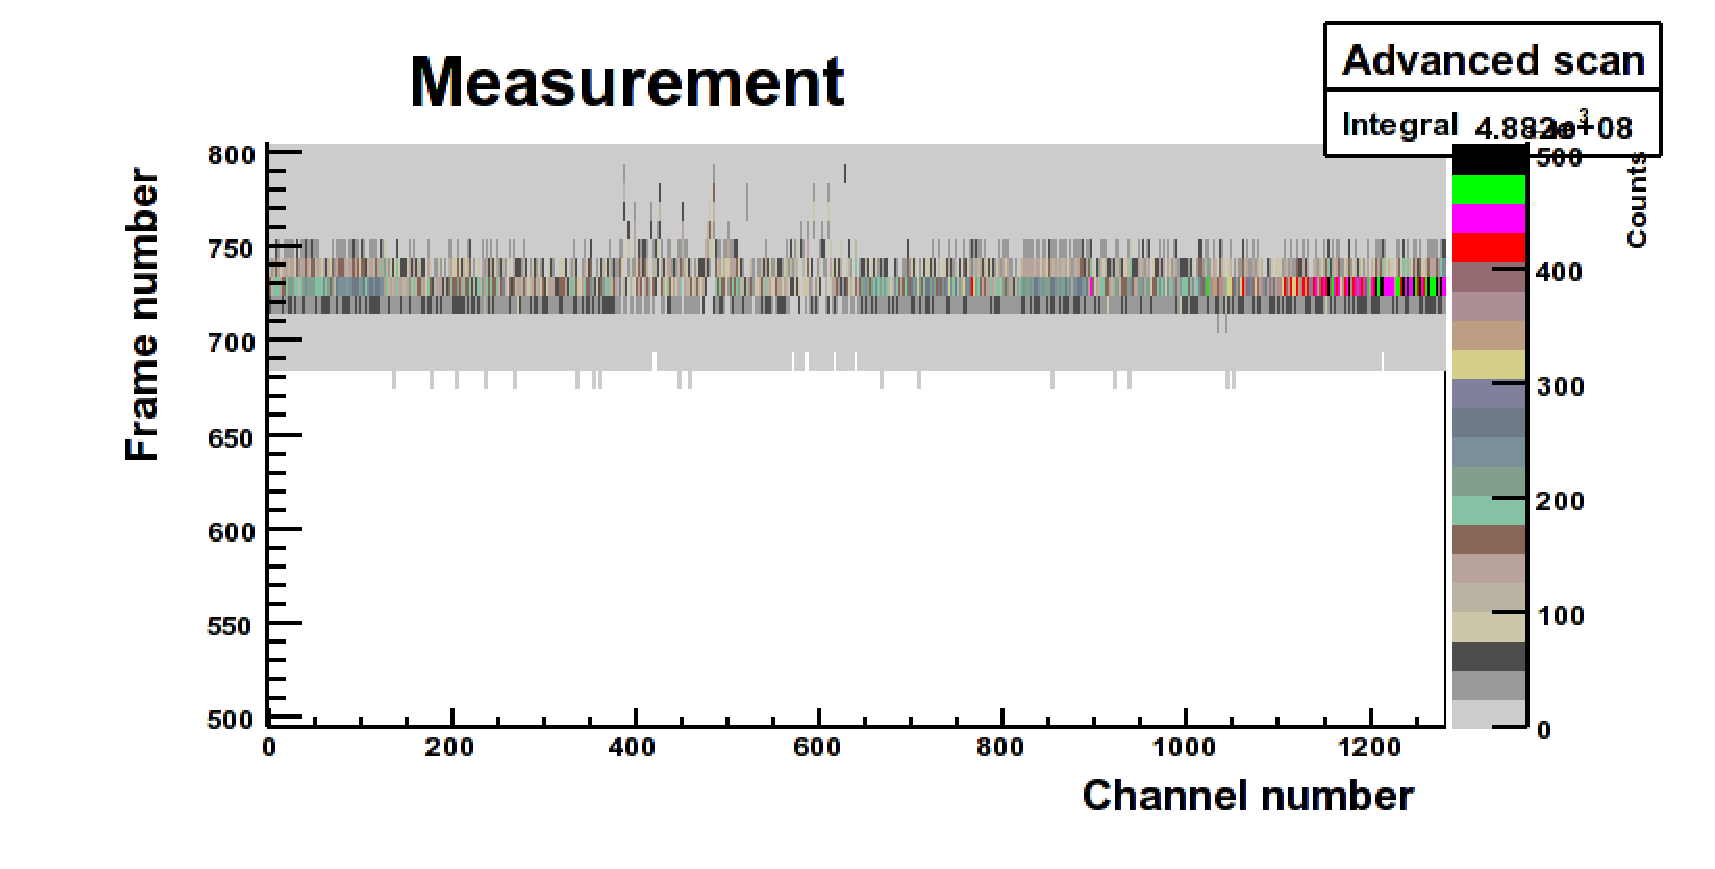
\includegraphics[width=\textwidth]{images/noise_thresholdscantrimmed}%
\lthtmlpictureZ
\lthtmlcheckvsize\clearpage}

\stepcounter{section}
\stepcounter{subsection}
{\newpage\clearpage
\lthtmlinlinemathA{tex2html_wrap_inline2813}%
$ \cdot$%
\lthtmlinlinemathZ
\lthtmlcheckvsize\clearpage}

\stepcounter{section}
\stepcounter{section}
\stepcounter{subsection}

\end{document}
